\begin{frame}
    \begin{center}
        \small
        Волгоградский Государственный Технический Университет \\
        Факультет электроники и вычислительной техники \\
        Кафедра физики \\
        \vspace{1.5cm}
        Выпускная работа на тему: \\
        \normalsize
        \textbf{Моделирование структуры абрикосовских вихрей в 
            сверхпроводниках типа 1,5} \\
        \vspace{1.5cm}
        \small
        Автор работы --- студент Ф-469 Голубев А. В. \\
        Научный руководитель --- д.ф.--м.н. Завьялов Д. В. \\
        \vspace{\fill}
        Волгоград \the\year
    \end{center}
\end{frame}

\begin{frame}
    \frametitle{Цель}
    \begin{itemize}
        \item исследование появления сверхпроводимости типа 1,5;
        \item исследования случая многополосной сверхпроводимости;
        \item теоретический анализ модели;
        \item моделирование структуры абрикосовских вихрей;
    \end{itemize}
\end{frame}

\begin{frame}
    \frametitle{Актуальность работы}
    \begin{itemize}
        \item широкие возможностями применения сверхпроводников в 
            современной микроэлектронике;
        \item высокотемпературные сверхпроводники;
        \item малая изученность физики данного процесса;
        \item перспективность в исследовании смешанного состояния;
    \end{itemize}
\end{frame}

\begin{frame}
    \frametitle{Фазовая диаграмма}
    \begin{figure}[h]
        \center
        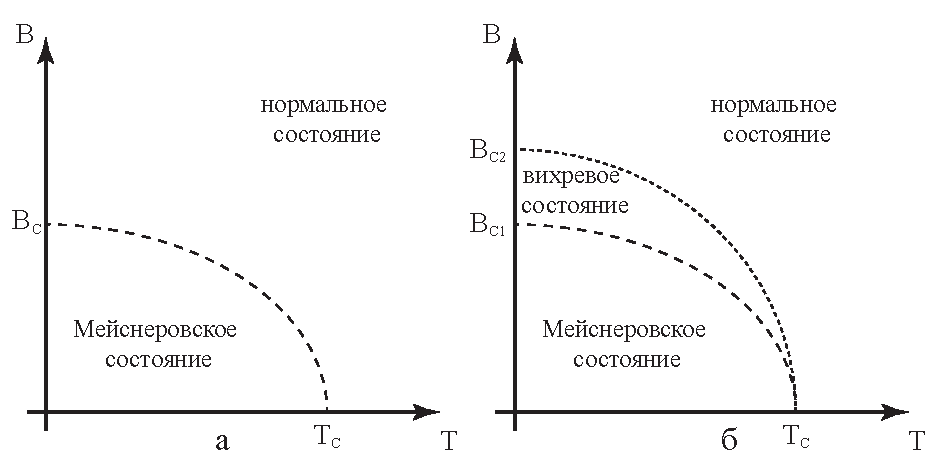
\includegraphics[width=1.0\linewidth]{img_01}
        \caption{Фазовая диаграмма состояния сверхпроводников 1-го (а) и 
            2-го (б) рода}
    \end{figure}
\end{frame}

\begin{frame}
    \frametitle{Фазовая диаграмма магнитных фаз}
    \begin{figure}[h]
        \center
        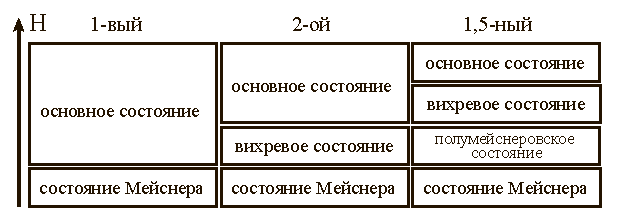
\includegraphics[width=1.0\linewidth]{1-02}
        \caption{Сравнение фазовых диаграмм магнитных фаз чистых 
            сверхпроводников первого, второго и полуторного рода при нулевой 
            температуре.}
    \end{figure}
\end{frame}

\begin{frame}
    \frametitle{Двухкомпонентная модель Гинзбурга-Ландау}
    \begin{gather}
        F = \frac{1}{2}\sum\limits_{a=1,2}\left[ 
            \left|\left( \nabla + ie\vec{A}\right)\psi_a\right|^2 + 
            \left( 2\alpha_a + \beta_a |\psi_a|^2 \right)|\psi_i|^2 \right] 
            + \nonumber \\ + \frac{1}{2}\left( \nabla\times\vec{A} \right)^2 - 
            \eta|\psi_1||\psi_2|\cos(\theta_2-\theta_1)
    \end{gather}
\end{frame}

\begin{frame}
    \frametitle{Метод моделирования структуры вихрей}
    \begin{gather}
        \left( \nabla f \right)_{i,i+1} = \frac{f(i+1)-f(i)}{h} \\
        B_{i,i+1,j,j+1} = \frac{1}{h^2}\oint\limits_{\omega} 
            \vec{A} \cdot d\vec{r}
    \end{gather}
    \begin{figure}[h]
        \center
        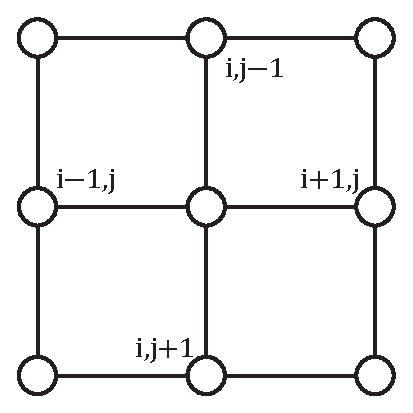
\includegraphics[width=0.5\linewidth]{scheme}
        \caption{Схема дискретизации используемая в методе конечных разностей, 
            (а) градиентов и (б) магнитного потока.}
    \end{figure}
\end{frame}

\begin{frame}
    \frametitle{Результаты модельного эксперимента}
    \framesubtitle{Поперечное сечение вихрей}
    \begin{figure}[h]
        \begin{minipage}[h]{0.75\linewidth}
            \center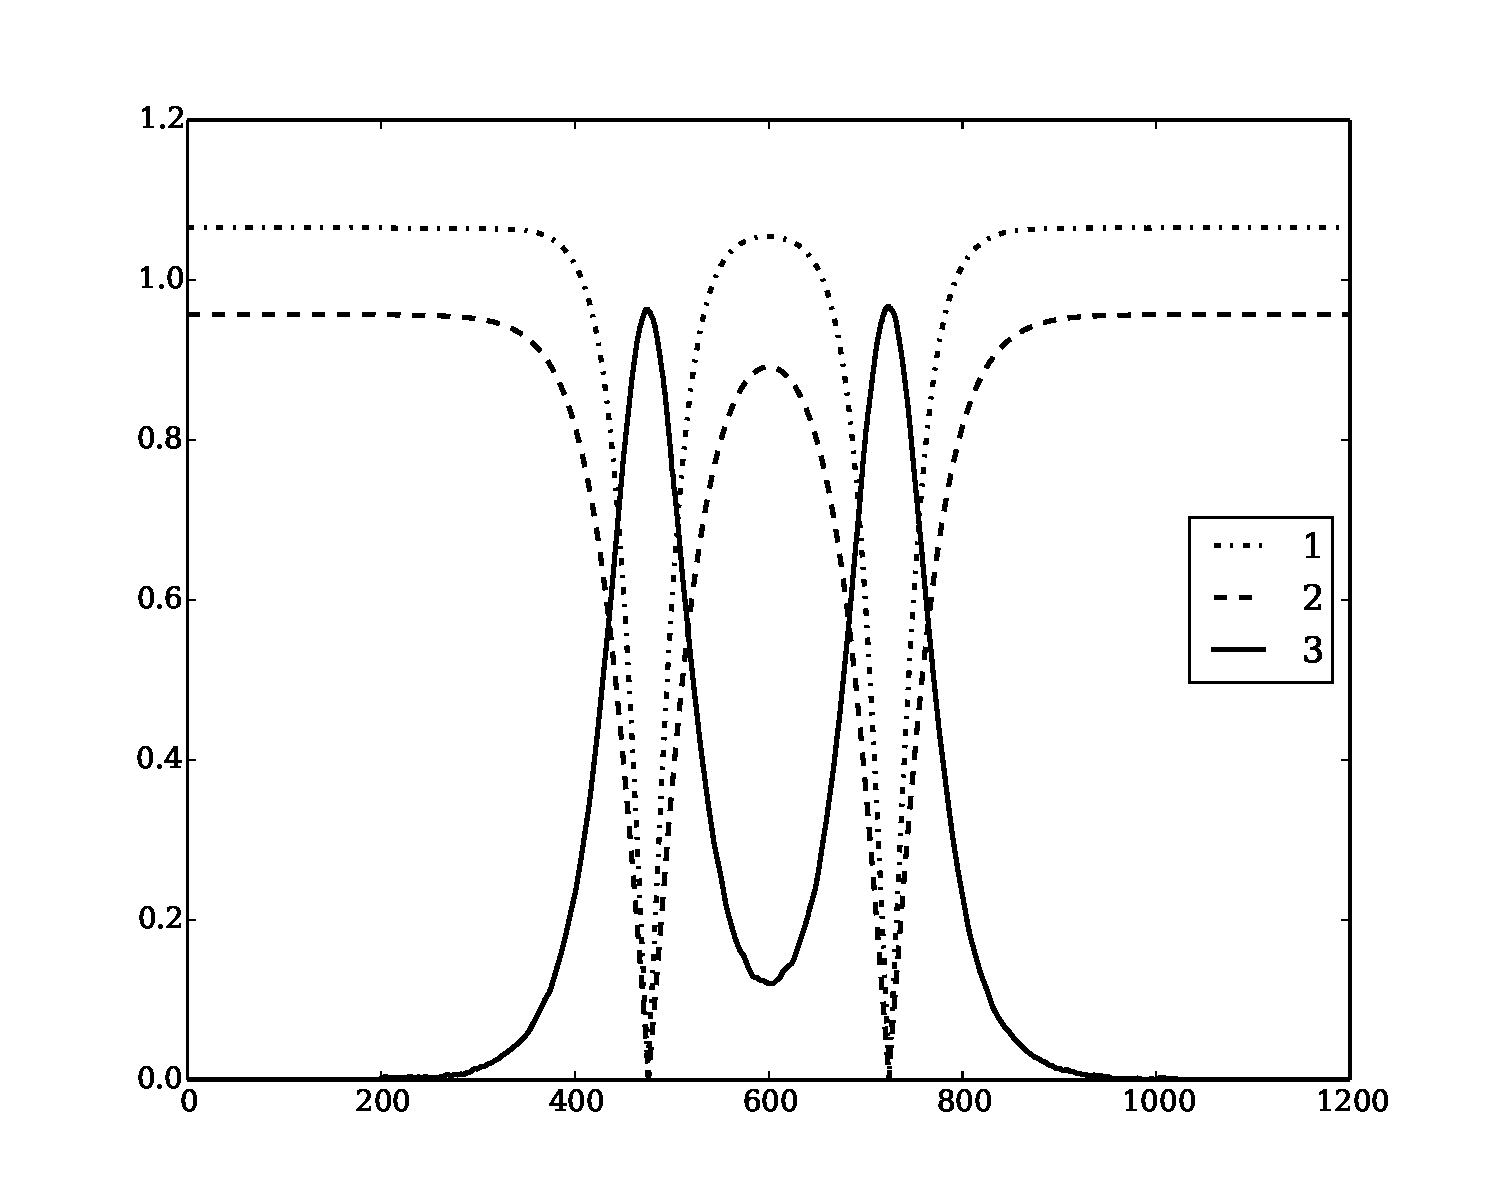
\includegraphics[width=1.1\linewidth]{band_profile}
        \end{minipage}
        \begin{minipage}[h]{0.15\linewidth}
            \( 1 \) -- \( \abs{\psi_1}^2 \), \\ 
            \( 2 \) -- \( \abs{\psi_2}^2 \), \\
            \( 3 \) -- \( B \).
        \end{minipage}
    \end{figure}
\end{frame}

\begin{frame}
    \frametitle{Результаты модельного эксперимента}
    \framesubtitle{Распределение магнитного поля (\( B \))}
    \begin{figure}[h]
        \begin{minipage}[h]{0.49\linewidth}
            \center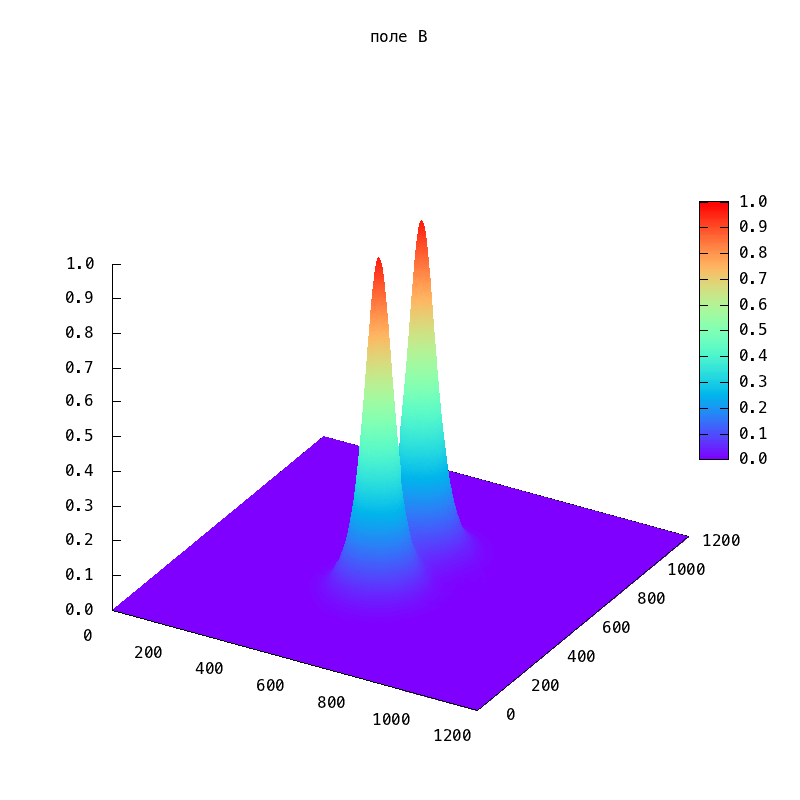
\includegraphics[width=1.1\linewidth]{3d_B}
        \end{minipage}
        \hfill
        \begin{minipage}[h]{0.49\linewidth}
            \center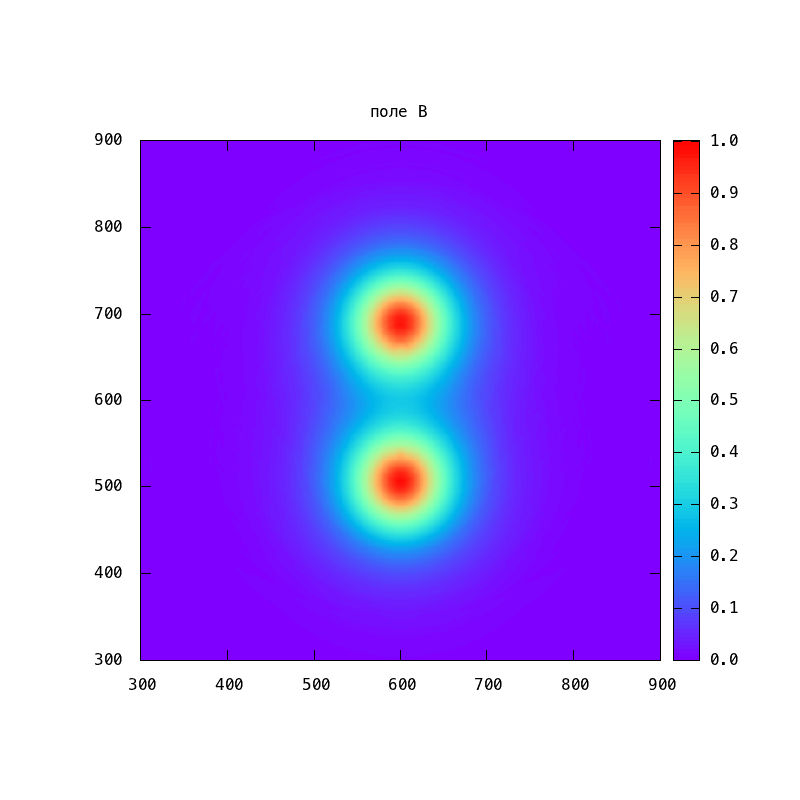
\includegraphics[width=1.1\linewidth]{map_B}
        \end{minipage}
    \end{figure}
\end{frame}

\begin{frame}
    \frametitle{Результаты модельного эксперимента}
    \framesubtitle{Характерный вид энергии взаимодействия первой зоны в 
        сверхпроводнике (\( \abs{\psi_1}^2 \)-компонента).}
    \begin{figure}[h]
        \begin{minipage}[h]{0.49\linewidth}
            \center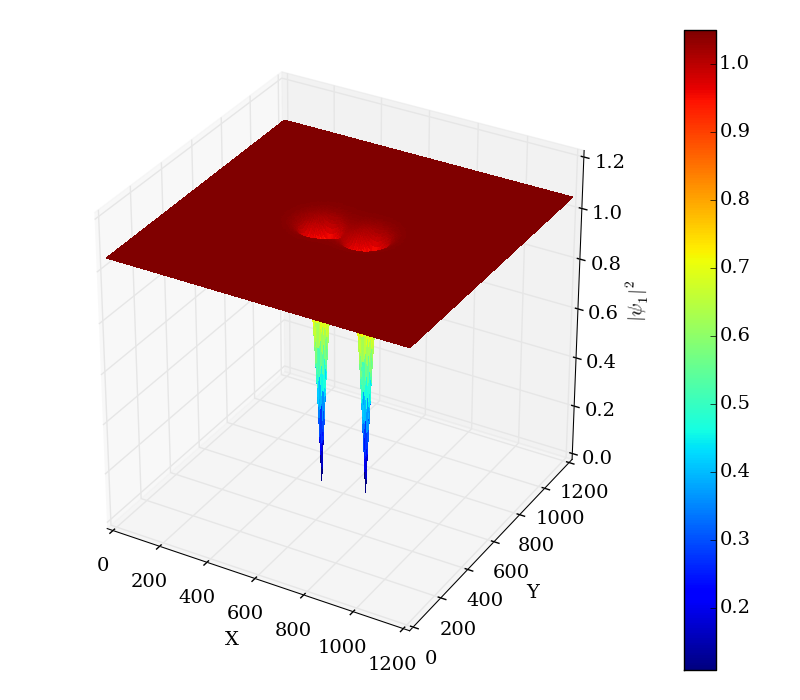
\includegraphics[width=1.1\linewidth]{3d_F1}
        \end{minipage}
        \hfill
        \begin{minipage}[h]{0.49\linewidth}
            \center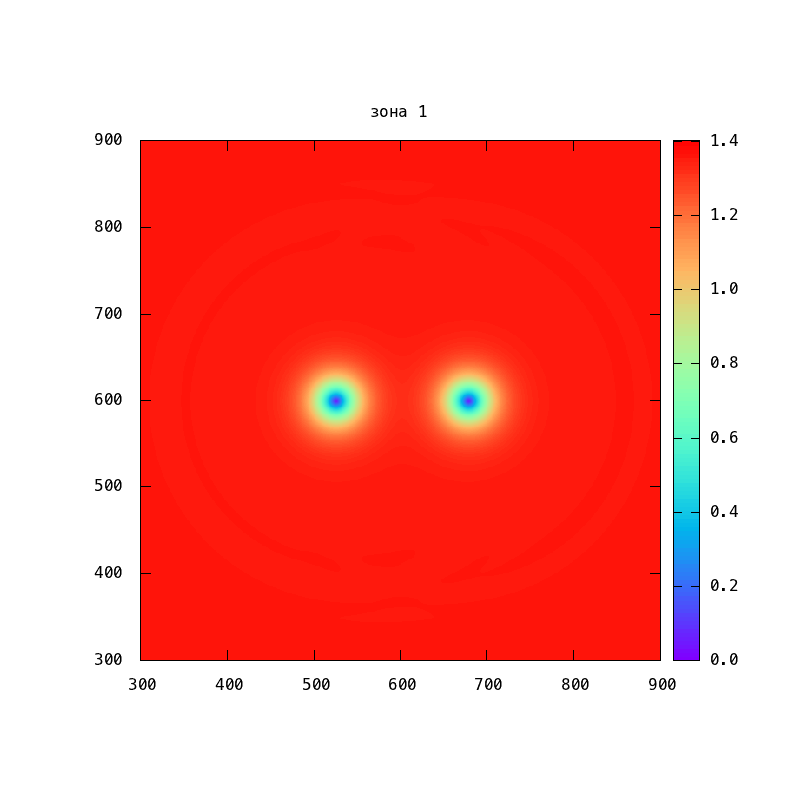
\includegraphics[width=1.1\linewidth]{map_F1}
        \end{minipage}
    \end{figure}
\end{frame}

\begin{frame}
    \frametitle{Результаты модельного эксперимента}
    \framesubtitle{Характерный вид энергии взаимодействия первой зоны в 
        сверхпроводнике (\( \abs{\psi_2}^2 \)-компонента).}
    \begin{figure}[h]
        \begin{minipage}[h]{0.49\linewidth}
            \center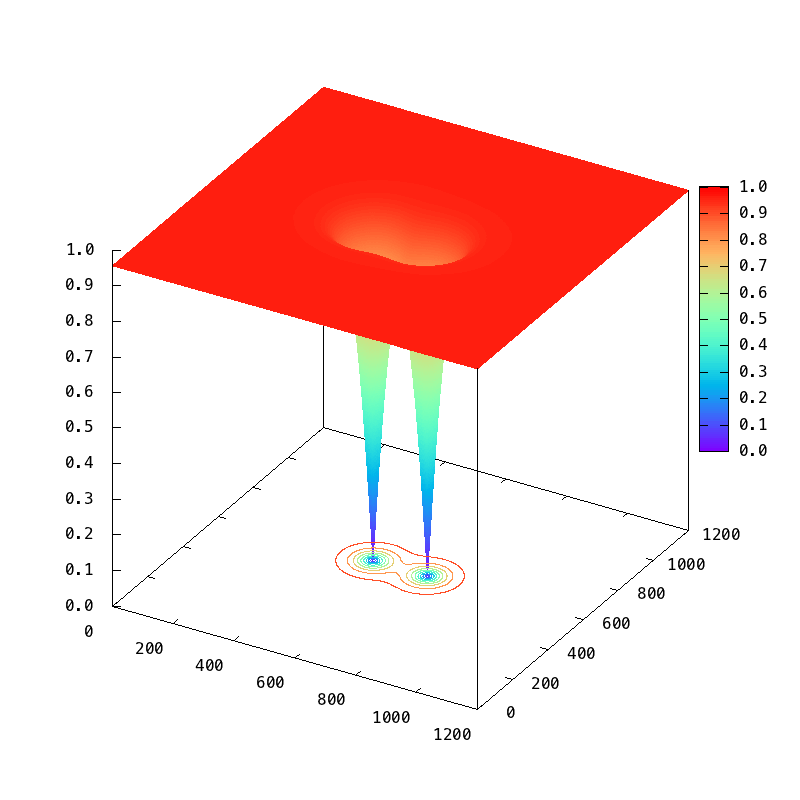
\includegraphics[width=1.1\linewidth]{3d_F2}
        \end{minipage}
        \hfill
        \begin{minipage}[h]{0.49\linewidth}
            \center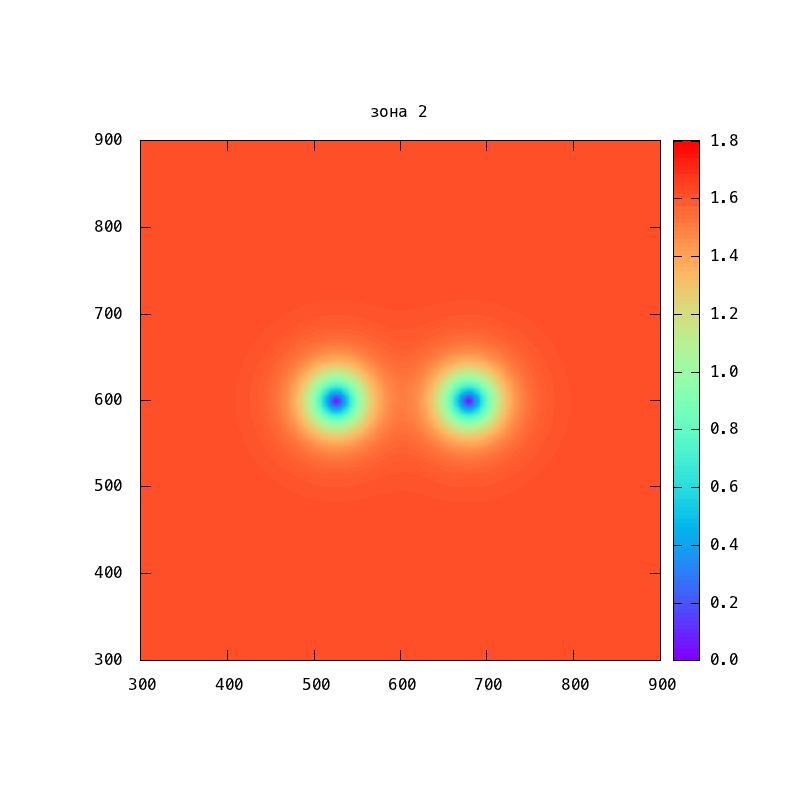
\includegraphics[width=1.1\linewidth]{map_F2}
        \end{minipage}
    \end{figure}
\end{frame}